% Options for packages loaded elsewhere
\PassOptionsToPackage{unicode}{hyperref}
\PassOptionsToPackage{hyphens}{url}
%
\documentclass[
]{book}
\usepackage{amsmath,amssymb}
\usepackage{lmodern}
\usepackage{ifxetex,ifluatex}
\ifnum 0\ifxetex 1\fi\ifluatex 1\fi=0 % if pdftex
  \usepackage[T1]{fontenc}
  \usepackage[utf8]{inputenc}
  \usepackage{textcomp} % provide euro and other symbols
\else % if luatex or xetex
  \usepackage{unicode-math}
  \defaultfontfeatures{Scale=MatchLowercase}
  \defaultfontfeatures[\rmfamily]{Ligatures=TeX,Scale=1}
\fi
% Use upquote if available, for straight quotes in verbatim environments
\IfFileExists{upquote.sty}{\usepackage{upquote}}{}
\IfFileExists{microtype.sty}{% use microtype if available
  \usepackage[]{microtype}
  \UseMicrotypeSet[protrusion]{basicmath} % disable protrusion for tt fonts
}{}
\makeatletter
\@ifundefined{KOMAClassName}{% if non-KOMA class
  \IfFileExists{parskip.sty}{%
    \usepackage{parskip}
  }{% else
    \setlength{\parindent}{0pt}
    \setlength{\parskip}{6pt plus 2pt minus 1pt}}
}{% if KOMA class
  \KOMAoptions{parskip=half}}
\makeatother
\usepackage{xcolor}
\IfFileExists{xurl.sty}{\usepackage{xurl}}{} % add URL line breaks if available
\IfFileExists{bookmark.sty}{\usepackage{bookmark}}{\usepackage{hyperref}}
\hypersetup{
  pdftitle={Repositório Digital das Humanidades (PT-BR)},
  pdfauthor={Leonardo F. Nascimento; Eric Brasil; Tarssio Barreto; Vítor Mussa; Daniel Mendes; Outro},
  hidelinks,
  pdfcreator={LaTeX via pandoc}}
\urlstyle{same} % disable monospaced font for URLs
\usepackage{longtable,booktabs,array}
\usepackage{calc} % for calculating minipage widths
% Correct order of tables after \paragraph or \subparagraph
\usepackage{etoolbox}
\makeatletter
\patchcmd\longtable{\par}{\if@noskipsec\mbox{}\fi\par}{}{}
\makeatother
% Allow footnotes in longtable head/foot
\IfFileExists{footnotehyper.sty}{\usepackage{footnotehyper}}{\usepackage{footnote}}
\makesavenoteenv{longtable}
\usepackage{graphicx}
\makeatletter
\def\maxwidth{\ifdim\Gin@nat@width>\linewidth\linewidth\else\Gin@nat@width\fi}
\def\maxheight{\ifdim\Gin@nat@height>\textheight\textheight\else\Gin@nat@height\fi}
\makeatother
% Scale images if necessary, so that they will not overflow the page
% margins by default, and it is still possible to overwrite the defaults
% using explicit options in \includegraphics[width, height, ...]{}
\setkeys{Gin}{width=\maxwidth,height=\maxheight,keepaspectratio}
% Set default figure placement to htbp
\makeatletter
\def\fps@figure{htbp}
\makeatother
\setlength{\emergencystretch}{3em} % prevent overfull lines
\providecommand{\tightlist}{%
  \setlength{\itemsep}{0pt}\setlength{\parskip}{0pt}}
\setcounter{secnumdepth}{5}
\usepackage{booktabs}
\ifluatex
  \usepackage{selnolig}  % disable illegal ligatures
\fi
\usepackage[]{natbib}
\bibliographystyle{apalike}

\title{Repositório Digital das Humanidades (PT-BR)}
\author{Leonardo F. Nascimento\footnote{UFBA - Laboratório de Humanidades Digitais, \href{mailto:leofn@ufba.br}{\nolinkurl{leofn@ufba.br}}} \and Eric Brasil\footnote{UNILAB - LABHDUFBA, \href{mailto:profericbrasil@unilab.edu.br}{\nolinkurl{profericbrasil@unilab.edu.br}}} \and Tarssio Barreto\footnote{UFBA - Laboratório de Humanidades Digitais, \href{mailto:tarssioesa@gmail.com}{\nolinkurl{tarssioesa@gmail.com}}} \and Vítor Mussa\footnote{UFRJ/PPGSA/DTA - LABHDUFBA, \href{mailto:vtrmussa@gmail.com}{\nolinkurl{vtrmussa@gmail.com}}} \and Daniel Mendes\footnote{UFRJ - PATHS, \href{mailto:daniel_mnds34@hotmail.com}{\nolinkurl{daniel\_mnds34@hotmail.com}}} \and Outro\footnote{UFRJ - PPGCS, \href{mailto:vmussa@gmail.com}{\nolinkurl{vmussa@gmail.com}}}}
\date{2021-04-27}

\begin{document}
\maketitle

{
\setcounter{tocdepth}{1}
\tableofcontents
}
\hypertarget{apresentauxe7uxe3o}{%
\chapter{Apresentação}\label{apresentauxe7uxe3o}}

A ideia desta obra foi reunir esforços de diferentes pesquisadores e instituições na elaboração de scripts para coletar - de modo automatizado - a produção intelectual dos principais congressos e eventos das áreas das humanidades.

Além disso, nós tivemos como objetivo mais amplo enfatizar a importância do desenvolvimento de habilidades computacionais por parte dos pesquisadores em todos os campos das humanidades.

Os scripts, as bases de dados e todos os documentos estão disponíveis e poderão ser baixados com apenas um clique. O acervo servirá para a realização de investigações sobre os mais variados aspectos e ampliar, com isso, o conhecimento sobre a produção acadêmica, científica e intelectual do Brasil das ciências humanas e sociais ao longo de décadas.

Para o lancamento, nós escolhemos o \href{https://dhcenternet.org/initiatives/day-of-dh/2021}{Dia Internacional das Humanidades Digitais} em 29/04/2021.

Ao compartilhar nas redes, pedimos que usem a hashtag \textbf{\#dayofdh21}

\begin{figure}
\centering

\includegraphics[width=0.35\textwidth,height=\textheight]{./img/dayofdh.jpg}
\caption{Símbolo do \#dayofdh21}
\end{figure}

\hypertarget{webscraping-e-ciuxeancias-sociais}{%
\chapter{Webscraping e ciências sociais}\label{webscraping-e-ciuxeancias-sociais}}

\hypertarget{por-que-automatizar}{%
\section{Por que automatizar?}\label{por-que-automatizar}}

\hypertarget{como-comeuxe7ar}{%
\section{Como começar?}\label{como-comeuxe7ar}}

\hypertarget{pruxf3s-e-contras}{%
\section{Prós e contras}\label{pruxf3s-e-contras}}

\hypertarget{pruxe9-requisitos}{%
\chapter{Pré-requisitos}\label{pruxe9-requisitos}}

\hypertarget{r-e-rstudio}{%
\section{R e Rstudio}\label{r-e-rstudio}}

\hypertarget{python}{%
\section{Python}\label{python}}

\hypertarget{anpuh}{%
\chapter{ANPUH}\label{anpuh}}

\hypertarget{o-que-uxe9-anpuh}{%
\section{O que é ANPUH?}\label{o-que-uxe9-anpuh}}

A \href{https://anpuh.org.br/index.php}{Associação Nacional de História, Anpuh}, fundada em 1961, inicialmente destinada aos docentes de cursos de graduação e pós-graduação. Em 1993, a ANPUH ampliou sua base para todoa os profissionais de história.

\begin{quote}
A cada dois anos, a ANPUH realiza o Simpósio Nacional de História, o maior e mais importante evento da área de história no país e na América Latina\footnote{\href{https://anpuh.org.br/index.php/quem-somos}{Anpuh-Quem somos}}.
\end{quote}

Desenvolvemos scripts diferentes para dois tipos de conjuntos de dados relacionados à Associação Nacional de História.

\begin{itemize}
\item
  Anais-Anpuh: script para raspagem de todos os trabalhos publicados nos Anais dos Simpósio Nacionais de História entre 1963 e 2017, disponíveis no site da Anpuh.
\item
  anpuh-scraper: script para raspagem dos resumos (e demais informações) de todos os trabalhos aprovados para todos os simpósios temáticos dos SNH nos aos de 2013, 2015, 2017 e 2019.
\end{itemize}

\hypertarget{anais-anpuh}{%
\section{Anais-Anpuh}\label{anais-anpuh}}

\href{https://github.com/LABHDUFBA/Anais-Anpuh}{Clique aqui para acessar o repositório no Github}.

\hypertarget{scripts-de-raspagem}{%
\subsection{Scripts de raspagem}\label{scripts-de-raspagem}}

Esse script realiza a raspagem dos trabalhos em PDF de todos os Simpósios Nacionais da Anpuh entre 1963 até 2017, disponíveis atualmente na site da associação, que podem ser \href{https://anpuh.org.br/index.php/documentos/anais}{acessados aqui}.

Escrito em \href{https://www.python.org/}{Python 3.8}, o script utiliza as seguintes bibliotecas e módulos

\begin{itemize}
\tightlist
\item
  \textbf{urllib.requests}: módulo do Python para acessar urls. \href{https://docs.python.org/pt-br/3/library/urllib.request.htmll}{Saiba mais.}
\item
  \textbf{os}: módulo do Python que permite manipular funções do sistema operacional. \href{https://docs.python.org/pt-br/3/library/os.html}{Saiba mais.}
\item
  \textbf{bs4}: \href{https://www.crummy.com/software/BeautifulSoup/bs4/doc/}{Beautiful Soup} é uma biblioteca Python para extrair dados de arquivos HTML e XML.
\item
  \textbf{re}: \href{https://docs.python.org/pt-br/3/library/re.html}{Regular Expressions} é um módulo do Python para operar com expressões regulares.
\item
  \textbf{pandas}: \href{https://pandas.pydata.org/}{Pandas} é uma biblioteca escrita em Python para manipulação e análise de dados.
\item
  \textbf{wget}: \href{https://pypi.org/project/wget/}{Wget} é uma biblioteca escrita em Python para realizar downloads.
\end{itemize}

O script tem o seguinte funcionamento quando executado:

\begin{itemize}
\tightlist
\item
  Cria pasta para salvar os PDFs, após verificar se a mesma não existe no local: \texttt{Anais\ Anpuh\textgreater{}\ pdf} utilizando módulo \texttt{os}.
\item
  Acessa a URL dos Anais com a biblioteca \texttt{urllib} e realiza a análise do HTML da mesma com a biblioteca \texttt{BeautifulSoup};
\item
  Cria uma lista de eventos a partir da página principal;
\item
  Acessa as páginas de cada evento contidas na lista criada anteriormente através de uma iteração;
\item
  Em cada item da lista de eventos, o script busca todos os papers da primeira página e cria uma nova lista. Nessa lista de papers de uma dada página o script realizará as seguintes ações:

  \begin{itemize}
  \tightlist
  \item
    encontrar as informações de cada paper;
  \item
    inclui essas informações em uma lista (que depois gerará um CSV com os dados);
  \item
    busca se há pdf disponível e se ele não é repetido faz download do PDF
  \item
    Após realizar essas ações para todos os itens de uma página, busca a próxima página de papers do evento, se não houver, passa para o próximo evento e repete as ações em um \emph{loop} até o último evento disponível.
  \end{itemize}
\end{itemize}

\hypertarget{dados}{%
\subsection{Dados}\label{dados}}

O script retorna para o usuário \textbf{todos os pdfs disponíveis em todas as páginas de todos os Simpósios Nacionais da Anpuh desde 1963 até 2017}. São criadas pastas com o número de cada evento para o armazenamento dos arquivos em PDF.

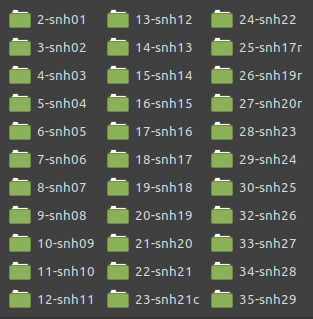
\includegraphics{img/pastas.png}

É importante notar que muitos papers não estão com pdf disponível no site, assim como nas edições mais antigas encontramos arquivos que contém vários papers num único PDF.

O script também gera um arquivo \textbf{CSV} (\emph{comma-separated values}) contendo os seguintes valores para cada paper: Autor(es)/Instituições,Título, Tipo, Evento, Ano, Link do Arquivo. Esse arquivo pode ser aberto como uma planilha e trabalhado em banco de dados.

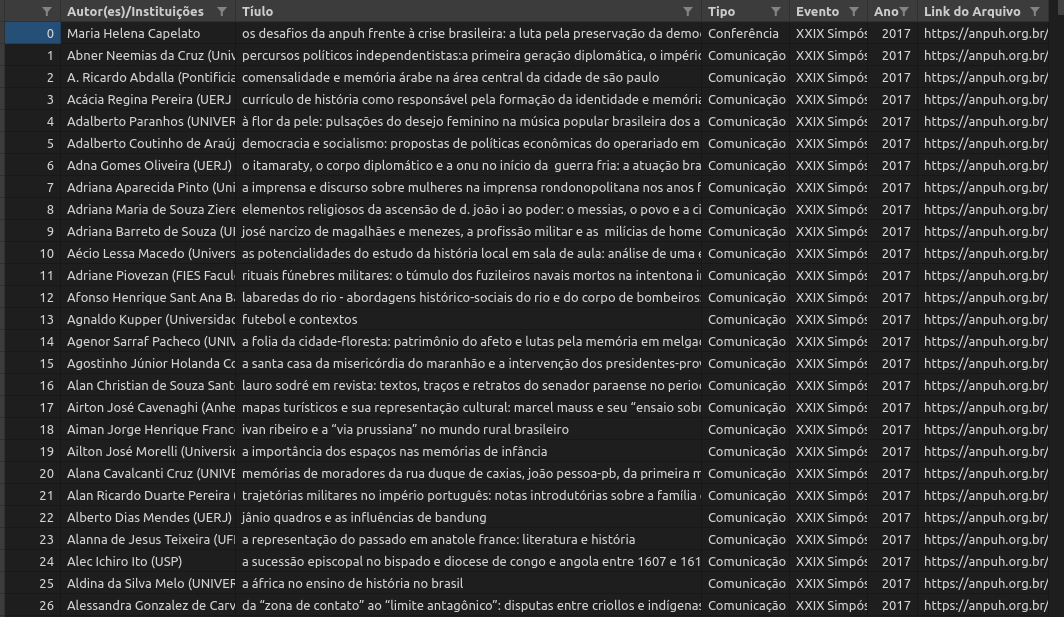
\includegraphics{img/ex_csv1.png}

\hypertarget{anpuh-scraper}{%
\section{anpuh-scraper}\label{anpuh-scraper}}

\href{https://github.com/LABHDUFBA/anpuh-scraper}{Clique aqui para acessar o repositório no Github}.

\hypertarget{scripts-de-raspagem-1}{%
\subsection{Scripts de raspagem}\label{scripts-de-raspagem-1}}

\emph{Raspador dos resumos dos Simpósios Nacionais de História da \href{https://anpuh.org.br}{Associação Nacional de História - Anpuh}. O programa raspa todos os resumos dos SNH 27, 28, 29 e 30, respectivamente dos anos de 2013, 2015, 2017 e 2019}
Escrito em \href{https://www.python.org/}{Python 3.8}, o script utiliza as seguintes bibliotecas e módulos

\begin{itemize}
\tightlist
\item
  \textbf{urllib.requests}: módulo do Python que ajuda a acessar urls.
  \href{https://docs.python.org/pt-br/3/library/urllib.request.htmll}{Saiba mais.}
\item
  \textbf{bs4}: \href{https://www.crummy.com/software/BeautifulSoup/bs4/doc/}{Beautiful Soup} é uma biblioteca Python para extrair dados de arquivos HTML e XML.
\item
  \textbf{pandas}: \href{https://pandas.pydata.org/}{Pandas} é uma biblioteca escrita em Python para manipulação e análise de dados.
\end{itemize}

O script tem o seguinte funcionamento quando executado:

Pergunta ao usuário que ano pretende raspar e se deseja incluir um novo ano à lista.
Após a criação da lista com os anos escolhidos pelo usuário, o script acessa cada uma das páginas com as listas dos STs nos sites de cada evento;
Acessa cada ST, encontra os dados de todos os resumos e passa para o ST seguinte;
Após terminar um ST, passa para o próximo evento e executa as mesmas função;
Todos os dados são inseridos em um DataFrame em Pandas e ao final são salvos no formato CSV.

\hypertarget{dados-1}{%
\subsection{Dados}\label{dados-1}}

O script retorna para o usuário um \textbf{CSV (\emph{comma-separated values}) com os dados de todos os trabalhos aceitos nos Simpósio Temáticos dos SNH 27, 28, 29 e 30}.

O CSV contém as seguintes variáveis para cada resumo:

\texttt{Ano,\ Evento,\ Cidade,\ ST,\ Coordenadores,\ Autor(es)/Instituições,\ Título,\ Resumo}

Esse arquivo pode ser aberto como uma planilha e trabalhado em banco de dados.

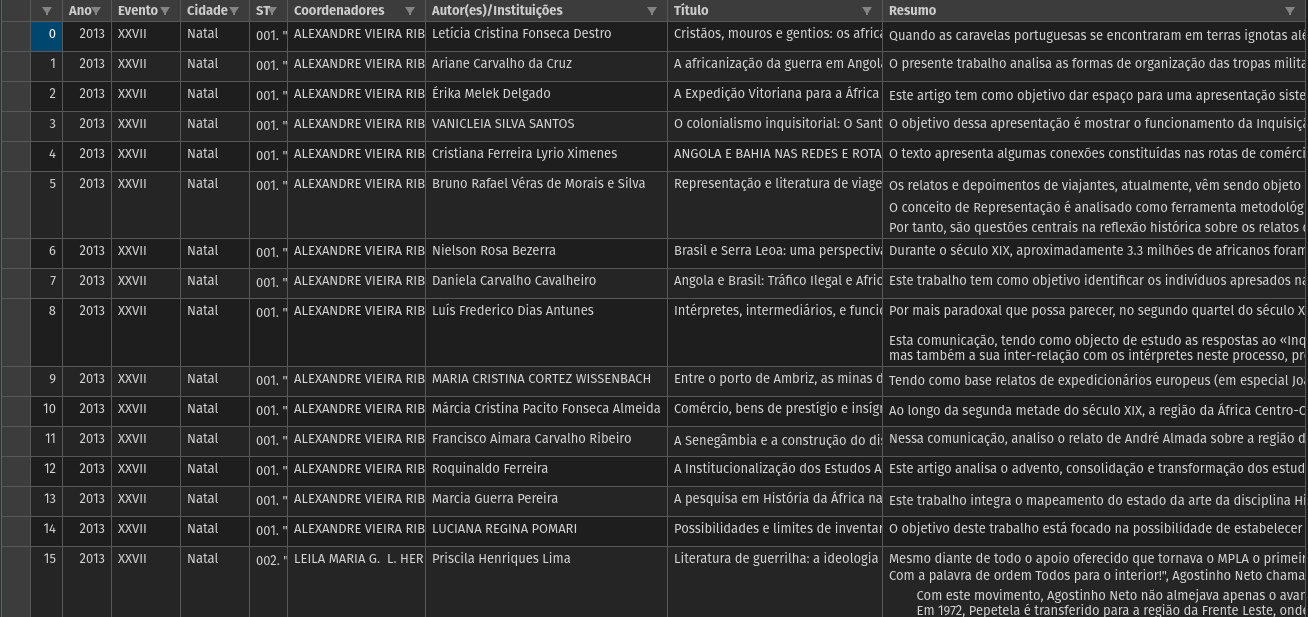
\includegraphics{img/ex_csv2.png}

\hypertarget{anpocs}{%
\chapter{ANPOCS}\label{anpocs}}

\hypertarget{o-que-uxe9-a-anpocs}{%
\section{O que é a ANPOCS?}\label{o-que-uxe9-a-anpocs}}

A \href{http://anpocs.com/}{Associação Nacional de Pós-Graduação e Pesquisa em Ciências Sociais (ANPOCS)} é uma entidade de direito privado sem fins lucrativos que reúne centenas de centros de pós-graduação e de pesquisa em antropologia, ciência política, relações internacionais e sociologia de todo o Brasil. Ela é formada, portanto, por instituições, em vez de pesquisadores individuais.

A associação organiza os \emph{Encontros Anuais da ANPOCS}, que consistem em congressos cujo número médio de participantes é de 1500 pesquisadores. Esses encontros estão entre os fóruns mais relevantes para as ciências sociais no Brasil.

Diante disso, desenvolvemos o \texttt{anpocs-scraper} -- \href{https://github.com/vmussa/anpocs-scraper}{disponível aqui} --, um raspador que permite coletar de forma automatizada os dados dos resumos dos trabalhos apresentados nos encontros de 2019, 2020 e, futuramente, 2021. O raspador expressa mais uma iniciativa que busca contribuir para uma ciência aberta e transparente, facilitando o acesso aos dados dos congressos e contribuindo para a preservação da memória das ciências sociais brasileiras.

\hypertarget{script-de-raspagem}{%
\section{Script de raspagem}\label{script-de-raspagem}}

\hypertarget{anpocs-scraper}{%
\subsection{anpocs-scraper}\label{anpocs-scraper}}

\includegraphics{img/demo.gif}

O \texttt{anpocs-scraper} é um raspador dos dados dos \href{http://anpocs.com/index.php/encontros/apresentacao}{Encontros Anuais da ANPOCS} escrito em Python. Atualmente o código permite coletar:

\begin{itemize}
\item
  os dados de todos os resumos dos trabalhos apresentados em GT's e SPG's do \href{https://www.anpocs2020.sinteseeventos.com.br/}{44º Encontro Anual da ANPOCS}
\item
  os dados de todos os resumos dos trabalhos apresentados em ST's e SPG's do \href{http://anpocs.com/index.php/43-encontro-anual-2019/2750-encontros-anuais/43-encontro/2301-resumos-sts-e-spgs}{43º Encontro Anual da ANPOCS}
\end{itemize}

\hypertarget{instalauxe7uxe3o-e-modo-de-uso}{%
\subsection{Instalação e modo de uso}\label{instalauxe7uxe3o-e-modo-de-uso}}

Para instalar o raspador basta clonar o repositório, \href{https://github.com/vmussa/anpocs-scraper}{que se encontra aqui}, e instalar suas dependências:

\begin{verbatim}
git clone https://github.com/vmussa/anpocs-scraper
cd anpocs-scraper
python -m venv .venv && source .venv/bin/activate
pip install -r requirements.txt
\end{verbatim}

Para rodar o raspador, continue no repositório clonado e execute o código \texttt{main.py} com o Python:

\begin{verbatim}
python src/main.py
\end{verbatim}

\begin{quote}
Atenção → \textbf{para realizar esse procedimento, você precisa instalar o Google Chrome e o ChromeDriver}: \href{https://chromedriver.chromium.org/getting-started}{Clique aqui} para ler um tutorial sobre como instalar o ChromeDriver.
\end{quote}

\hypertarget{em-breve}{%
\subsection{Em breve}\label{em-breve}}

Futuramente o raspador abarcará todos os GT's e SPG's do encontro 45, cujos resumos dos trabalhos estarão disponíveis \href{https://www.anpocs2021.sinteseeventos.com.br/}{aqui}. Além disso, ele contará com um módulo de limpeza dos dados que fará o pré-processamento para a análise qualitativa e/ou computacional.

\hypertarget{dados-2}{%
\section{Dados}\label{dados-2}}

O programa exporta, para cada edição do congresso, uma tabela no formato CSV com as seguintes informações de cada trabalho apresentado:

\begin{quote}
\texttt{autores}, \texttt{titulo}, \texttt{resumo}, \texttt{sessao}, \texttt{id\_evento}
\end{quote}

A imagem abaixo ilustra o formato de uma das tabelas:

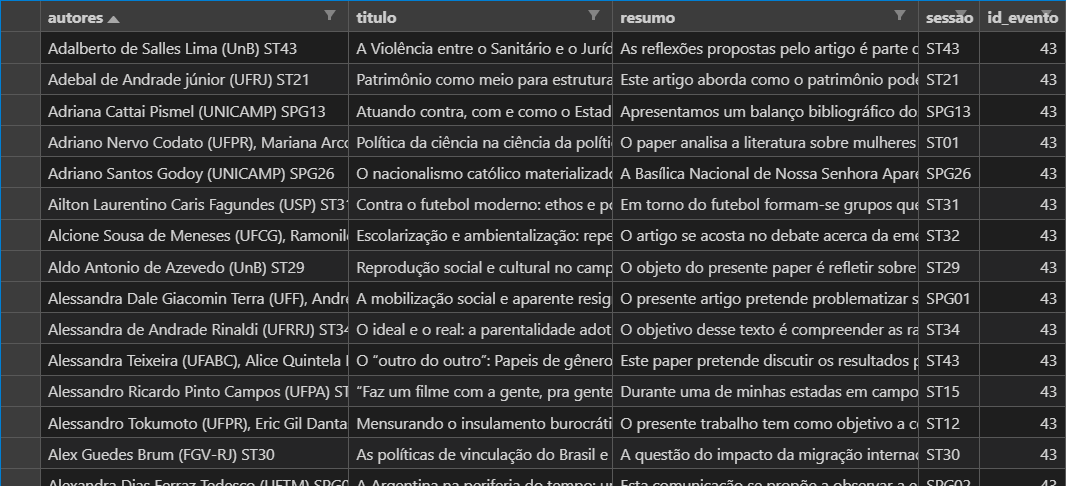
\includegraphics{img/anpocs_scraper_csv.png}

\hypertarget{compos}{%
\chapter{ComPos}\label{compos}}

\hypertarget{o-que-uxe9-a-compuxf3s}{%
\section{O que é a Compós?}\label{o-que-uxe9-a-compuxf3s}}

\hypertarget{script-de-raspagem-1}{%
\section{Script de raspagem}\label{script-de-raspagem-1}}

\hypertarget{dados-3}{%
\section{Dados}\label{dados-3}}

\hypertarget{referuxeancias-bibliogruxe1ficas}{%
\chapter{Referências Bibliográficas}\label{referuxeancias-bibliogruxe1ficas}}

AAAAAAAAAAAAAAA

\hypertarget{sobre-os-autores}{%
\chapter{Sobre os autores}\label{sobre-os-autores}}

\hypertarget{leo}{%
\section{Leo}\label{leo}}

\hypertarget{eric-brasil-ihlmunilab}{%
\section{Eric Brasil (IHLM/UNILAB)}\label{eric-brasil-ihlmunilab}}

Professor do curso de licenciatura em História e professor do Bacharelado Interdisciplinar em Humanidades no Instituto de Humanidades e Letras da Universidade da Integração Internacional da Lusofonia Afro-brasileira (IHL-UNILAB), campus dos Malês, Bahia.

Autor do livro A Corte em Festa: experiências negras em carnavais do Rio de Janeiro (1879-1888) (Editora Prismas, 2016).
Doutor (2016) e Mestre (2011) pelo Programa de Pós-Graduação em História Social da Universidade Federal Fluminense.

Vencedor do primeiro lugar no Concurso de Monografias Silvio Romero de 2011 e do segundo lugar em 2020, promovido pelo Centro Nacional de Folclore e Cultura Popular.

Pesquisador do Laboratório de Humanidades Digitais da UFBA. Membro do GT Nacional Emancipações e Pós-Abolição da Anpuh.
Tem experiência na área de História Social da Cultura, Humanidades e História Digital, Abolição da escravidão e o Pós-Abolição no Brasil e no Caribe, atuando principalmente nos seguintes temas: Carnaval, Cidadania, História Transnacional, Diáspora Africana, História das Afro-Américas, Hemerotecas e arquivos digitais, métodos digitais de pesquisa, linguagem de programação para a pesquisa em História, web scraping.

Foi professor de ensino fundamental, médio e pré-vestibular no Rio de Janeiro entre 2007 e 2017.

Currículos e redes acadêmicas

\href{https://ericbrasiln.github.io}{Webpage} - \href{http://lattes.cnpq.br/6853705640900524}{Lattes} - \href{\%22https://orcid.org/0000-0001-5067-8475}{Orcid} - \href{https://www.researchgate.net/profile/Eric_Brasil}{ResearchGate} - \href{https://unilab.academia.edu/EricBrasil}{Academia.edu}

\hypertarget{vuxedtor-mussa-dtappgsaufrj-e-labhdufbaufba}{%
\section{Vítor Mussa (DTA/PPGSA/UFRJ e LABHDUFBA/UFBA)}\label{vuxedtor-mussa-dtappgsaufrj-e-labhdufbaufba}}

Mestrando do Programa de Pós-Graduação em Sociologia e Antropologia (PPGSA) da Universidade Federal do Rio de Janeiro (UFRJ).

É membro do grupo de pesquisa Desenvolvimento, Trabalho e Ambiente (\href{https://www.nucleodta.org/inicio}{DTA-UFRJ}) e do Laboratório de Humanidades Digitais da Universidade Federal da Bahia (\href{http://www.labhd.ufba.br/}{LABHD-UFBA}).

Currículos e redes acadêmicas

\href{https://vmussa.github.io}{Webpage} - \href{http://lattes.cnpq.br/2934187748254130}{Lattes} - \href{https://www.researchgate.net/profile/Vitor-Mussa-2}{ResearchGate} - \href{https://www.linkedin.com/in/vmussa/}{LinkedIn} - \href{https://twitter.com/vitormussa}{Twitter}

\hypertarget{tarssio}{%
\section{Tarssio}\label{tarssio}}

\hypertarget{daniel-mendes-pathsufrj}{%
\section{Daniel Mendes (PATHS/UFRJ)}\label{daniel-mendes-pathsufrj}}

Graduando no curso de Bacharelado em Ciências Sociais do Instituto de Filosofia e Ciências Sociais (IFCS) da Universidade Federal do Rio de Janeiro (UFRJ).

É membro do grupo de pesquisa Núcleo de Pesquisa em Estratificação e Trajetórias Sociais (\href{https://www.facebook.com/paths.research/}{PATHS}).

Currículos e redes acadêmicas

\href{http://lattes.cnpq.br/9834413442426550}{Lattes} - \href{https://www.linkedin.com/in/daniel-mendes-251212176/}{LinkedIn} - \href{https://twitter.com/danielmnds34}{Twitter}

\hypertarget{gabriel-andrade-labhdufbaufba}{%
\section{Gabriel Andrade (LABHDUFBA/UFBA)}\label{gabriel-andrade-labhdufbaufba}}

Graduando no curso de Bacharelado em Engenharia de Computação da Escola Politécnica da Universidade Federal da Bahia (UFBA)

É desenvolvedor de software e membro do Laboratório de Humanidades Digitais da Universidade Federal da Bahia (\href{http://www.labhd.ufba.br/}{LABHD-UFBA}).

Currículos e redes acadêmicas

\href{https://gabrielsandrade.github.io}{Webpage} - \href{http://lattes.cnpq.br/4915378425369073}{Lattes} - \href{https://www.linkedin.com/in/gabriel-andrade-633996108}{LinkedIn} - \href{https://twitter.com/ga_brieell_}{Twitter}

\hypertarget{ajude-o-projeto}{%
\section{Ajude o projeto!}\label{ajude-o-projeto}}

\begin{figure}
\centering

\includegraphics[width=0.35\textwidth,height=\textheight]{C:/Users/Leonardo/Desktop/redhbr/img/btc.png}
\caption{bc1qmug7kcrw3kxklca7chy7c344d62gtc8fhqwnkw}
\end{figure}

  \bibliography{book.bib,packages.bib}

\end{document}
